\documentclass{beamer}

\usepackage{beamerthemesplit}
\usetheme{Warsaw}
\usepackage[utf8]{inputenc}

\title{Lisp}
\subtitle{'(Emacs Lisp)}
\author{Dimitri Fontaine}
\date{29 février 2012}

\begin{document}

\frame{\titlepage}

\begin{frame}[fragile]
  \frametitle{Emacs Lisp ?}

  \begin{center}
    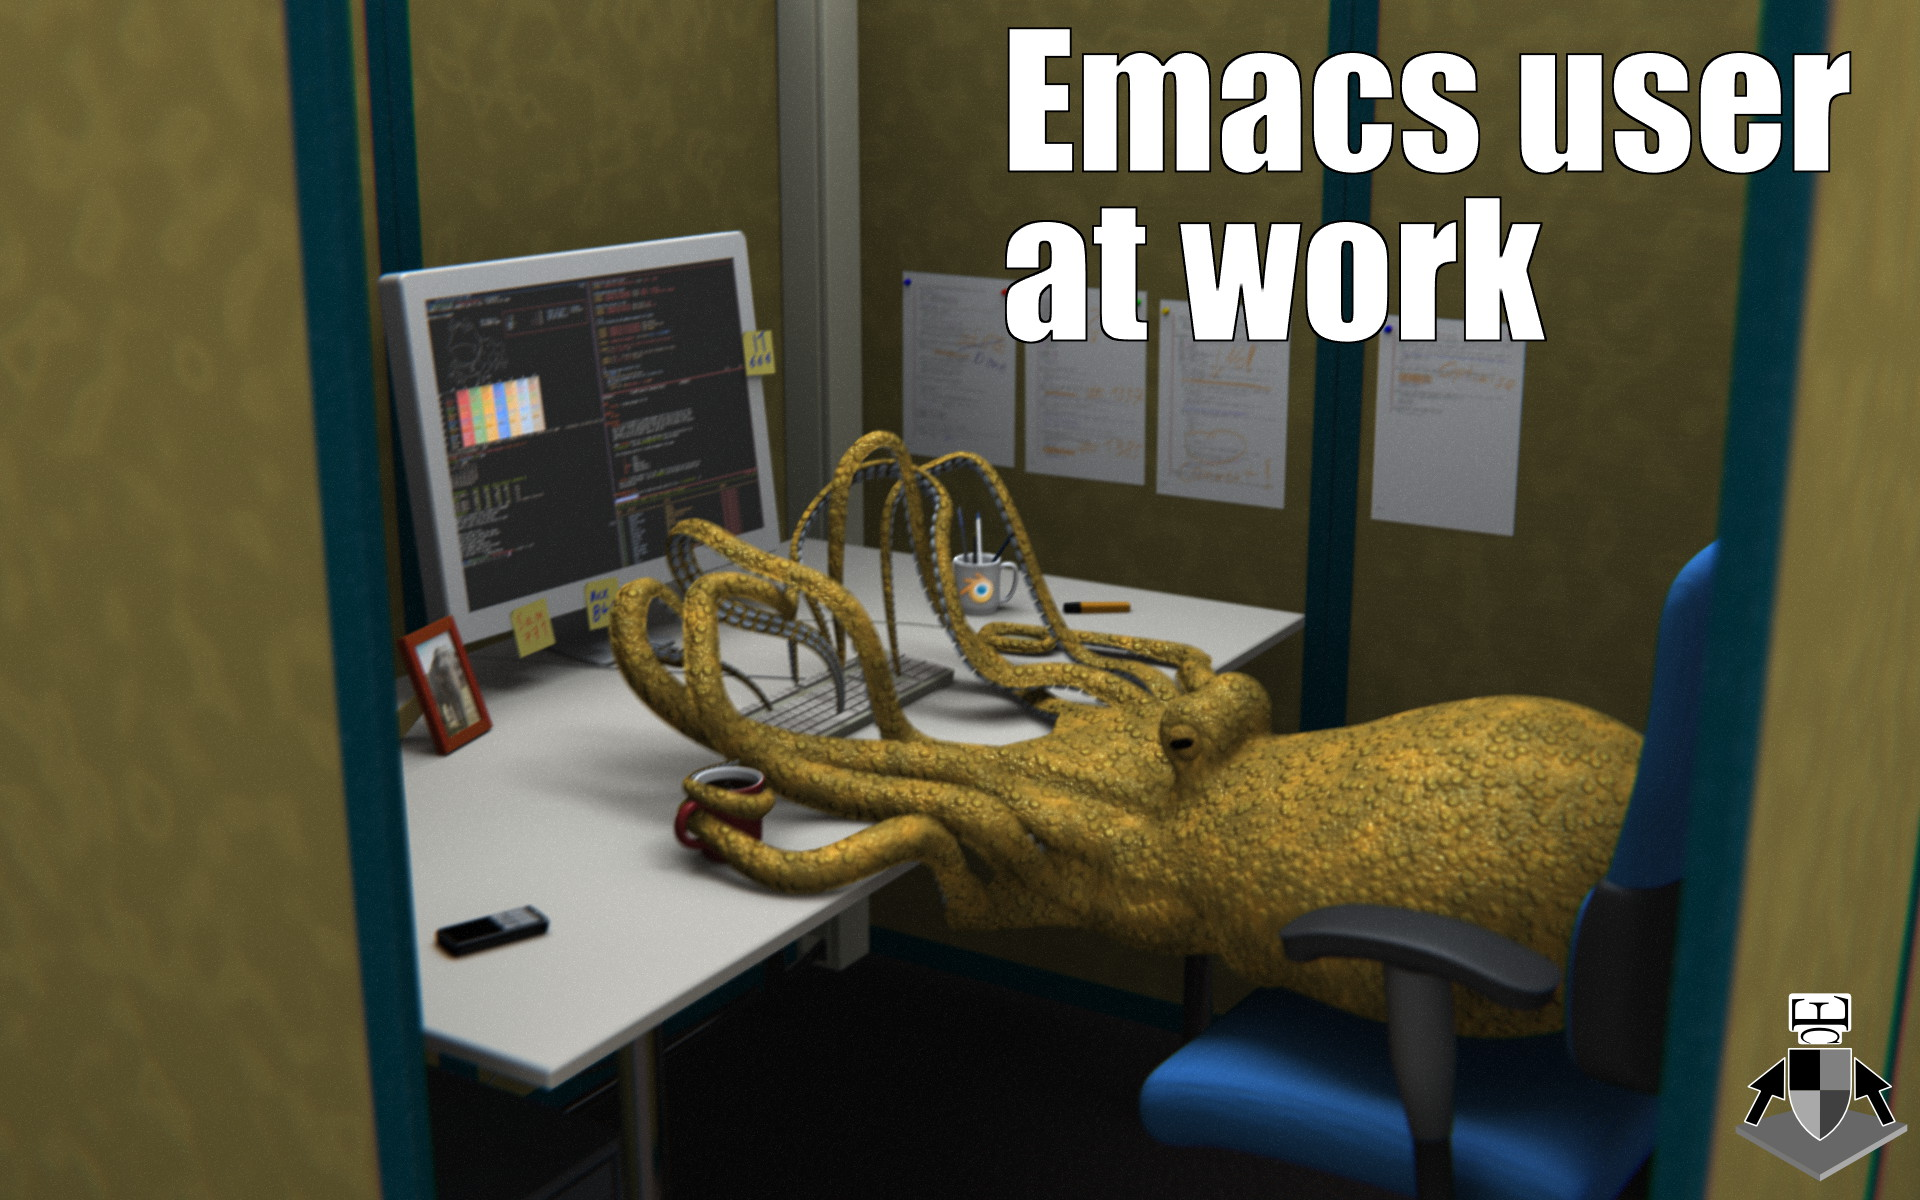
\includegraphics[height=2.7in]{emacs_user_at_work.jpeg}
  \end{center}
\end{frame}

\frame{
  \frametitle{Emacs Development Environment}

  Emacs inclue tout le nécessaire pour développer en Elisp, éditeur,
  documentation, compilateur, interprêteur, debugger interactif…

  \begin{itemize}
   \item \texttt{C-M-x} runs the command eval-defun
   \item \texttt{C-x C-e} runs the command eval-last-sexp
   \item \texttt{L} runs the command dired-do-load
   \item \texttt{M-x ielm} runs the command ielm
   \item \texttt{C-j} runs the command eval-print-last-sexp
  \end{itemize}
}

\begin{frame}[fragile]
  \frametitle{Lisp Syntax}

  La syntaxe Lisp est très simple, tellement simple qu'il faut s'y habituer :

\begin{example}[Syntaxe Emacs Lisp]
\begin{verbatim}
(defun dim:add-my-extra-load-paths (&optional paths)
  "define a list of paths to add to `load-path'
   and add each of them"
  (let ((dim:paths '("~/dev/emacs/el-get"
                     "~/dev/emacs.d")))
    (dolist (path (or paths dim:paths))
      (setq load-path (cons path load-path))))

(dim:add-my-extra-load-paths)
\end{verbatim}
\end{example}
\end{frame}
\begin{frame}[fragile]
  \frametitle{Lisp Syntax}

  D'autres exemples :

\begin{example}[Syntaxe Emacs Lisp]
\begin{verbatim}
 (defmacro until (cond &rest body)
    `(while (progn ,@body ,cond)))

  (defmacro when-running-debian (&rest body)
    "eval body only when running under debian"
    `(when (equal
  	  (lsb-release "Distributor ID") "Debian")
       ,@body))
\end{verbatim}
\end{example}

\end{frame}

\begin{frame}[fragile]
  \frametitle{Lisp Syntax}
  \begin{center}
    \url{http://www.lisperati.com/}

    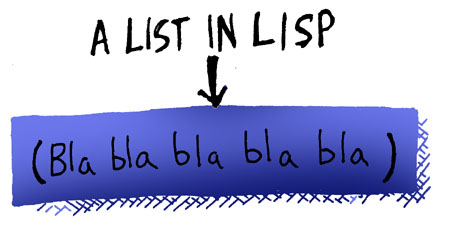
\includegraphics[height=1.4in]{lisp-list.jpg}
  \end{center}
\end{frame}

\begin{frame}[fragile]
  \frametitle{Lisp Syntax}
  \begin{center}
    \url{http://www.lisperati.com/}

    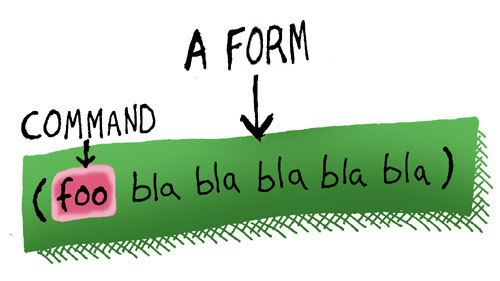
\includegraphics[height=1.4in]{lisp-form.jpg}
  \end{center}
\end{frame}

\begin{frame}[fragile]
  \frametitle{Lisp Syntax}
  \begin{center}
      \url{http://www.lisperati.com/}

    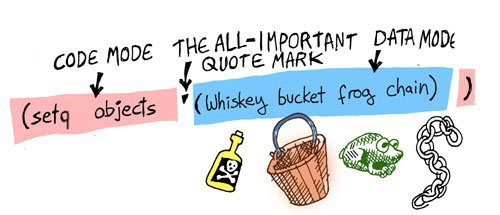
\includegraphics[height=1.4in]{game-objects.jpg}
  \end{center}
\end{frame}

\begin{frame}[fragile]
  \frametitle{Lisp Syntax}
  \begin{center}
    \url {http://www.lisperati.com/}

    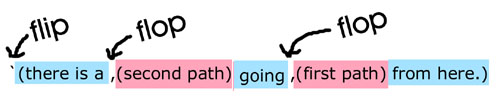
\includegraphics[height=0.7in]{back-quote.jpg}
  \end{center}
\end{frame}

\begin{frame}[fragile]
  \frametitle{Pourquoi tant de parenthèses ?}

  \begin{center}
    Est-ce vraiment spécifique à Lisp ?
  \end{center}

  \begin{example}[java]
\begin{verbatim}
closeButton.addActionListener(new ActionListener() {
    public void actionPerformed(ActionEvent event) {
        System.exit(0);
    }
});
\end{verbatim}
  \end{example}

  \begin{example}[C]
\begin{verbatim}
cmd->objectname =
   pstrdup(NameStr((
     ((Form_pg_conversion) GETSTRUCT(tup))->conname)));
\end{verbatim}
  \end{example}

\end{frame}

\frame{
  \frametitle{Lisp}

  Lisp a été découvert en 1960 et continue d'évoluer.

  Pour les curieux : \url{http://www.gigamonkeys.com/book/}

  \begin{itemize}
   \item Inclue les \textit{DSL} via les macros (cf. \texttt{loop})
   \item CLOS pour le développement object
   \item Grande famille (Common Lisp, Scheme, Emacs Lisp, …)
   \item Variables dynamiques et closures lexicales
   \item Seule famille de language à proposer les \textit{macros}
   \item Typage dynamique
   \item De nombreux types disponibles, pas seulement les \textit{listes}
   \item Gestion d'exception très avancée
   \item Continuations
  \end{itemize}
}

\frame{
  \frametitle{Emacs Lisp}

  Emacs inclue tout le nécessaire pour développer en Elisp, éditeur,
  documentation, compilateur, interprêteur, debugger interactif…

  \begin{itemize}
   \item Environnement interactif complet
   \item Documentation de référence
   \item Portabiblité étendue (Linux, Windows, MacOSX, Solaris, etc…)
   \item Interprêteur et compilateur (byte code)
   \item Intégration système (synchrone et asynchrone avancée)
   \item API riche, des milliers d'extensions (\texttt{cl.el})
   \item 36 ans d'histoire avec rétro compatibilité
  \end{itemize}
}

\end{document}
